\documentclass[letterpaper]{article}
\usepackage{enumitem}
\usepackage{geometry}
\usepackage{float}
\geometry{margin=1in}
\usepackage[protrusion=true,expansion=true]{microtype}
\usepackage[boxruled,linesnumbered,vlined,inoutnumbered]{algorithm2e}
\usepackage{amsmath}
\usepackage{placeins}
\usepackage[table,xcdraw]{xcolor}
\usepackage{amsthm}
\usepackage{amssymb}
\usepackage{afterpage}
\usepackage{mathtools}
\usepackage{soul}
\usepackage{mathrsfs}
\usepackage{soul}
\usepackage{natbib}
\usepackage{rotating}
\usepackage{textcomp, gensymb}
\usepackage{lscape}
\usepackage{array}
\usepackage{makecell}
\renewcommand\theadalign{bc}
\renewcommand\theadfont{\bfseries}
\renewcommand\theadgape{\Gape[4pt]}
\renewcommand\cellgape{\Gape[4pt]}
\usepackage{courier}
\usepackage{lipsum}
\usepackage{graphicx}
\usepackage{subcaption}
\usepackage[space]{grffile}
\usepackage{xcolor}
\definecolor{light-grey}{rgb}{0.9,0.9,0.9}
\definecolor{dark-red}{rgb}{0.7,0.0,0.1}
\definecolor{dark-blue}{rgb}{0,0,0.7}
\usepackage{environ}
\setcounter{tocdepth}{2}
\renewcommand{\contentsname}{Table of Contents}
\usepackage{hyperref}
\hypersetup{
    colorlinks, linkcolor={dark-blue},
    citecolor={dark-blue}, urlcolor={dark-blue}
}

% Used to show Python code
\usepackage{listings}
\lstdefinestyle{mystyle}{
    %backgroundcolor=\color{backcolour},   
    commentstyle=\color{dark-blue},
    keywordstyle=\color{magenta},
    numberstyle=\tiny\color{light-grey},
    %stringstyle=\color{codepurple},
    basicstyle=\ttfamily\footnotesize,
    breakatwhitespace=false,         
    breaklines=true,                 
    captionpos=b,                    
    keepspaces=true,                 
    numbers=left,                    
    numbersep=5pt,                  
    showspaces=false,                
    showstringspaces=false,
    showtabs=false,                  
    tabsize=2,
    basicstyle=\footnotesize, frame=tb,
    xleftmargin=.1\textwidth, xrightmargin=.1\textwidth
}
\lstset{style=mystyle}


\setlength{\parskip}{1em}
\newcommand{\HIGHLIGHT}[1]{\textcolor{blue}{\textbf{#1}}}
\newcommand{\TODO}[1]{\textcolor{red}{\textbf{#1}}}




\begin{document}
%-----------------
%	Final Project
%-----------------
\newpage
\begin{center}
	\begin{Large}
		COMPSCI 589 - Final Project - Spring 2024
	\end{Large}
	\\
	\HIGHLIGHT{Due May 10, 2024, 11:55 pm Eastern Time}
\end{center}
\addcontentsline{toc}{subsection}{\textbf{Final Project}}



\vspace{0.25in}
\section{Instructions}

\begin{itemize}
	\item \textbf{This final project should be done in groups of two students}. When making your submission on Gradescope, please do not forget to \href{https://help.gradescope.com/article/m5qz2xsnjy-student-add-group-members}{add all students who worked on this assignment}. Do that \underline{both} when submitting your code and your final report.
	\item We strongly recommend that you use \LaTeX~to prepare your submission. The assignment should be submitted on Gradescope as a PDF with marked answers via the Gradescope interface. The source code should be submitted via the Gradescope programming assignment as a .zip file. Include with your source code instructions for how to run your code.
	\item You may \textit{not} use any machine learning-specific libraries in your code, e.g., TensorFlow, PyTorch, or any machine learning algorithms implemented in scikit-learn. You may use libraries like numpy and matplotlib. If you are not certain whether a specific library is allowed, do ask us.
	\item All submissions will be checked for plagiarism using two independent plagiarism-detection tools. Renaming variable or function names, moving code within a file, etc., are all strategies that \textit{do not} fool the plagiarism-detection tools we use. \textcolor{red}{If you get caught, all penalties mentioned in the syllabus \textit{will} be applied---which may include directly failing the course with a letter grade of ``F''}.
	\item The tex file for this assignment (which you can use if you decide to write your solution in \LaTeX), as well as the datasets, can be found \href{https://people.cs.umass.edu/~bsilva/courses/CMPSCI_589/Spring2024/homeworks/final_project.zip}{here}.
	\item The automated system will not accept assignments after 11:55pm on May 10.
	\item Notice that you \underline{\textbf{cannot}} use your ``free late days'' on this assignment.
\end{itemize}


%---------------------------------------------
\newpage

\vspace{1cm}
\section{Final Project --- Overall Goals}

\begin{itemize}
	\item The goal of this final project is to compare the performance of different machine learning algorithms you implemented throughout the semester by testing them on four new, challenging datasets.
	\item By performing these comparisons, you will gain practical experience in selecting an algorithm (based on a given problem) and optimizing its hyper-parameters so that it works well. In addition, these analyses will give you insight into how to solve novel machine learning problems---problems where no one tells you which algorithms may work best nor how to adjust their hyper-parameters.
	\item \textbf{This project should be done in groups of two students}.
	\item \textbf{Notice that you may \ul{not} use existing machine learning libraries for this assignment: \textcolor{dark-red}{you \underline{\textit{must}} use the implementations that you or your partner designed throughout the semester}}.
	\item On each question below, please clearly indicate whose implementation was used; i.e., make sure that you explicitly mention the name of the student whose code was used to tackle each particular dataset.
	\item We expect the amount of time and effort you put into this assignment will be slightly \textit{less} than that required to solve one homework. The reason is that this final project will not require implementing new algorithms, other than the ones you already implemented during the semester. Also, you will be working in groups and so it should be easier to split up tasks evenly.
	      \vspace{0.5cm}
	\item \textcolor{dark-red}{\textbf{Alternative: ``Custom Project''}}. You may replace the tasks mentioned above with a ``custom project'' that is more closely aligned with your interests. It has to be ML-related and use some of the techniques we discussed in class. For reasons of fairness, this project \textit{cannot} be used as part of any other UMass activity for which you are given credit (e.g., other courses or independent studies). A custom project related to a research project that you are conducting with a UMass professor (or with anyone else) is acceptable if you are not already getting graded for it. If you would like to work on a custom project, please check with the instructor (bsilva@cs.umass.edu) if the custom project you have in mind would be acceptable. If the project is deemed acceptable, you should let the instructor know, \textit{before you start working on the project}, which tasks will be assigned to each student in the group.

\end{itemize}


%---------------------------------------------
\newpage


\section{Datasets}
\label{sec:datasets}

\textbf{\textcolor{blue}{As part of this final project, you will be analyzing four datasets.} }



\subsection{The Hand-Written Digits Recognition Dataset}
The goal, here, is to analyze 8x8 pictures of hand-written digits (see, e.g., Fig.~\ref{fig:digits}) and classify them as belonging to one of 10 possible classes. Each class is associated with one particular digit: $0, 1, \ldots, 9$. In this dataset, each instance is composed of $8 \times 8 = 64$ numerical attributes, each of which corresponding to the grayscale value of one pixel in the image being classified. This dataset is composed of 1797 instances.

\begin{figure}[!h]
	\centering
	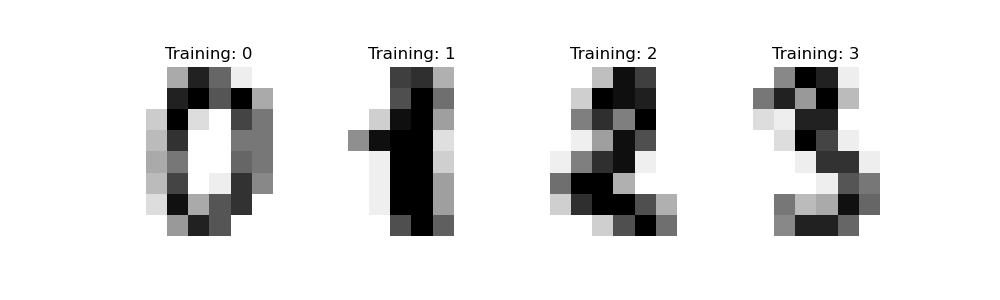
\includegraphics[width=0.8\columnwidth]{figures/digits.png}
	\caption{Examples of hand-written digits that you will be classifying.}
	\label{fig:digits}
\end{figure}

To access this dataset, and for sample code describing how to load and pre-process it, please visit \href{https://scikit-learn.org/stable/auto_examples/classification/plot_digits_classification.html}{Scikit-learn's website}. Further, please find below (in Fig.~\ref{fig:digits_loading}) a simple example of how to load this dataset; here, the instances are saved in \textit{digits\_dataset\_X} and their corresponding classes are saved in \textit{digits\_dataset\_y}.


\begin{figure}[h!]
	\centering
	\begin{lstlisting}[language=Python]
from sklearn import datasets
import numpy as np
import matplotlib.pyplot as plt

digits = datasets.load_digits(return_X_y=True)
digits_dataset_X = digits[0]
digits_dataset_y = digits[1]
N = len(digits_dataset_X)

# Prints the 64 attributes of a random digit, its class, 
# and then shows the digit on the screen
digit_to_show = np.random.choice(range(N),1)[0]
print("Attributes:", digits_dataset_X[digit_to_show])
print("Class:", digits_dataset_y[digit_to_show])
	
plt.imshow(np.reshape(digits_dataset_X[digit_to_show], (8,8)))
plt.show()	
\end{lstlisting}
	\caption{Example of how to load the Digits dataset from Scikit-learn, and how to show information about a random instance/digit in the dataset.}
	\label{fig:digits_loading}
\end{figure}

\afterpage{\clearpage}
\FloatBarrier



%---------------------------------------------
\newpage
\subsection{The Titanic Dataset}

On April 15, 1912, the largest passenger liner ever made collided with an iceberg during her maiden voyage. When the Titanic sank, it killed 1502 out of 2224 passengers and crew. One of the reasons the shipwreck resulted in such loss of life was that there were not enough lifeboats for the passengers and crew. Although luck was involved in surviving the sinking, some groups of people were more likely to survive than others.

The goal, here, is to predict whether a given person was likely to survive this tragedy. The dataset contains data corresponding to 887 real passengers of the Titanic. Each row represents one person. The columns describe different attributes of the person, including whether they survived, their age, their passenger class, sex, and the fare they paid. The target class (\textit{Survived}) is encoded in the first column of the dataset.  \href{https://people.cs.umass.edu/~bsilva/courses/CMPSCI_589/Spring2024/homeworks/final_project.zip}{The Titanic dataset can be found in this assignment's zip file}. Notice that this dataset combines both numerical and categorical attributes.



\subsection{The Loan Eligibility Prediction Dataset}

Here, the goal is to automatically (and accurately) predict whether a given person should qualify for a loan. Each instance is described by 13 attributes, including the Loan\_ID, the gender of the applicant, whether the applicant is married, their income, information about their credit history, etc. The binary target class to be predicted is \textit{Loan\_Status}: whether a given applicant's request for a loan was approved or not. Notice that this dataset contains 8 categorical attributes, 4 numerical attributes, and a Loan\_ID attribute. There is a total of 480 instances in the dataset. \href{https://people.cs.umass.edu/~bsilva/courses/CMPSCI_589/Spring2024/homeworks/final_project.zip}{The Loan dataset can be found in this assignment's zip file}.



\subsection{The Oxford Parkinson's Disease Detection Dataset}

This dataset is composed of a range of biomedical voice measurements from 31 people, 23 of whom are patients with Parkinson's disease. Each row in the dataset corresponds to the voice recording from one of these individuals. Each attribute corresponds to the measurement of one specific property of the patient's voice---for example, their average vocal frequency or several measures of frequency variation. The goal, here, is to predict whether a particular person is healthy or whether it is a patient with Parkinson's. The binary target class to be predicted is \textit{Diagnosis}: whether the patient is healthy (class 0) or a patient with Parkinson's (class 1). There are 195 instances in this dataset. All 22 attributes are numerical. \href{https://people.cs.umass.edu/~bsilva/courses/CMPSCI_589/Spring2024/homeworks/final_project.zip}{The Parkinson's dataset can be found in this assignment's zip file}.


\vspace{1cm}
\noindent\rule{\textwidth}{1pt}
$\star$ Before running experiments to analyze each dataset above, manually verify if it makes sense to consider all features/attributes. E.g., should the learning algorithm be given the identifier of a loan? Or the name of a person? If you choose to remove one or more attributes, explain why you decided to do so in your report.

\noindent $\star$ Notice that some of the datasets above include both categorical and numerical attributes. Algorithms such as neural networks (as well as others) require numerical inputs. The standard way of converting categorical inputs to numerical inputs is by using by one-hot encoding technique. For a quick and high-level introduction to one-hot encoding, as well as examples on how to use Scikit's libraries to perform this type of conversion, please visit this \href{https://datagy.io/sklearn-one-hot-encode}{website}.



%---------------------------------------------
\newpage
\section{Experiments and Analyses}

\HIGHLIGHT{For each dataset, you should}:

\begin{enumerate}
	\item Evaluate the performance of \textcolor{dark-red}{at least two algorithms} you studied and/or implemented during the semester (e.g., $k$-NN, Decision Trees, standard Naive Bayes, Random Forests, Neural Networks, etc).\footnote{Evaluating more algorithms will give you extra credit. See Section \ref{sec:extra_credit}.} You should discuss which algorithms you decided to test on each dataset and why.
	\item You should evaluate the performance of each algorithm on a given dataset in terms of its accuracy and F1 score. Use stratified cross-validation with $k=10$.
	\item To obtain the best performance possible, you should carefully adjust the \textit{hyper-parameters} of each algorithm when deployed on a dataset. For example, you may have to experiment with different values of $k$ when optimizing the $k$-NN algorithm; different values of $ntree$ when optimizing a Random Forest; different architectures and regularization parameters when optimizing a neural network; etc.
	\item Given the observation above, you should \ul{first show, in a table, the performance of each algorithm (on a given dataset) under a few selected hyper-parameters}. You should evaluate at least 3 hyper-parameter settings. After analyzing the performance of each algorithm under different hyper-parameters, identify the best hyper-parameter setting---that is, the set of hyper-parameters that resulted in the best performance for the corresponding algorithm on a particular dataset.
	\item \ul{For each dataset, and considering the best hyper-parameter setting for each selected algorithm, construct relevant learning curves and/or graphs}. These should be similar to the learning curves/graphs you constructed in the homework relevant to the particular algorithm you are evaluating. For example, if you choose to deploy a Random Forest to tackle one of the datasets, construct a graph relating its performance and the number of trees in the ensemble; if you choose to use a neural network, construct a learning curve showing the value of the cost function, $J$, as a function of the number of training instances presented to the network. Assuming that you evaluate two algorithms on each of the four datasets, these analyses should result in (at least) 8 graphs. \ul{Briefly discuss and interpret these graphs}. For example: Why do you think a particular algorithm may be converging to a poor local optimum when deployed on a given dataset? Why do you think a specific algorithm performs better on datasets containing only numerical attributes? and so on.
\end{enumerate}

After conducting the analyses above for each dataset, you should summarize your results in a table. In particular, you should create a table showing, for each dataset, the performance (accuracy and F1-score) of each of the algorithms. Your table should look like Table \ref{fig:results_table}. You should highlight (in gray) the cells that indicate which algorithm had the highest performance---according to each of the metrics---on each dataset. In the example shown in Table \ref{fig:results_table}, for instance, we can see that, when analyzing Dataset 1, Algorithm 1 had the highest accuracy but Algorithm 2 had the highest F1 score.


\begin{table}[h!]
	\centering
	\begin{tabular}{|c|cc|cc|cc|cc|}
		\hline
		            & \multicolumn{2}{c|}{Dataset 1}                & \multicolumn{2}{c|}{Dataset 2} & \multicolumn{2}{c|}{Dataset 3}                & \multicolumn{2}{c|}{Dataset 4}                                                                                                                                                       \\ \hline
		            & \multicolumn{1}{c|}{Accuracy}                 & F1-Score                       & \multicolumn{1}{c|}{Accuracy}                 & F1-Score                       & \multicolumn{1}{c|}{Accuracy}                 & F1-Score                 & \multicolumn{1}{c|}{Accuracy}                 & F1-Score                 \\ \hline
		Algorithm 1 & \multicolumn{1}{c|}{\cellcolor[HTML]{C0C0C0}} &                                & \multicolumn{1}{c|}{}                         &                                & \multicolumn{1}{c|}{}                         & \cellcolor[HTML]{C0C0C0} & \multicolumn{1}{c|}{}                         &                          \\ \hline
		Algorithm 2 & \multicolumn{1}{c|}{}                         & \cellcolor[HTML]{C0C0C0}       & \multicolumn{1}{c|}{}                         &                                & \multicolumn{1}{c|}{}                         &                          & \multicolumn{1}{c|}{\cellcolor[HTML]{C0C0C0}} & \cellcolor[HTML]{C0C0C0} \\ \hline
		Algorithm 3 & \multicolumn{1}{c|}{}                         &                                & \multicolumn{1}{c|}{\cellcolor[HTML]{C0C0C0}} & \cellcolor[HTML]{C0C0C0}       & \multicolumn{1}{c|}{}                         &                          & \multicolumn{1}{c|}{}                         &                          \\ \hline
		...         & \multicolumn{1}{c|}{}                         &                                & \multicolumn{1}{c|}{}                         &                                & \multicolumn{1}{c|}{\cellcolor[HTML]{C0C0C0}} &                          & \multicolumn{1}{c|}{}                         &                          \\ \hline
	\end{tabular}
	\caption{Example of how the table summarizing your final results look like.}
	\label{fig:results_table}
\end{table}

To facilitate the task of creating this table on \LaTeX, please visit this \href{https://www.tablesgenerator.com}{website}. We have created a template for generating tables similar to the one shown above. This template can be found in the \textit{table\_results.tgn} file, provided to you as part of this assignment's  \href{https://people.cs.umass.edu/~bsilva/courses/CMPSCI_589/Spring2024/homeworks/final_project.zip}{zip file}. You can load this template on the website mentioned above (File $\rightarrow$ Load Table) and complete the table with your results.

% \afterpage{\clearpage}
% \FloatBarrier


%---------------------------------------------
\newpage

\section{Extra Credit}
\label{sec:extra_credit}

\textbf{There are four ways in which we may receive extra credit on this assignment.} If you choose to work on any of the tasks below, please clearly indicate in your report,  \textcolor{dark-red}{\textbf{in red}}, which specific tasks you are working on for extra credit. Describe what you did as part of that task and discuss the corresponding results. Any source code you develop should be included in your Gradescope submission.

\noindent \HIGHLIGHT{\textcolor{dark-red}{(Extra Points \#1: 10 Points)}}
You may earn up to 10 extra points if you analyze all four datasets using an additional algorithm. That is, in this case you would be evaluating more than just two algorithms on each dataset.

\noindent \HIGHLIGHT{(Extra Points \#2: 10 Points)}
You may earn up to 10 extra points if you select a new \textit{challenging} dataset and evaluate the performance of different algorithms on it. A challenging dataset should necessarily include both categorical and numerical attributes and have more than two classes; or it should be a dataset where you have to classify images.

\noindent \HIGHLIGHT{\textcolor{dark-red}{ (Extra Points \#3: 15 Points) }}
You may earn up to 15 extra points if you \textit{combine} different algorithms and construct an ensemble. For instance, you could create an ensemble composed of three neural networks (each with a different architecture) and a random forest. The process of training the ensemble would be as described in class---each algorithm would be trained based on its own bootstrap dataset, etc. The final predictions would then be determined via majority voting. Evaluate your ensemble algorithm on all four datasets discussed in Section \ref{sec:datasets}.


\noindent \HIGHLIGHT{(Extra Points \#4: 15 Points)}
You may earn up to 15 extra points if you implement a new type of algorithm---a non-trivial variant of one of the algorithms studied in class. If you choose to do so, you should evaluate its performance on all four datasets discussed in Section \ref{sec:datasets}.

\section{Analyses}

Algorithms we are using:
\begin{itemize}
	\item kNN (by Nhan Lai)
	\item Random Forest (by Bang Cao)
	\item Neural Network (by Bang Cao)
	\item Neural Network Ensemble
	\item Linear Regression
\end{itemize}

\subsection{Digits Dataset}

All attributes are numerical so no need for one hot encode.

\subsection*{Random Forest}
\begin{itemize}
	\item \text{Split criterion: Information Gain}
	\item $min\_size\_split = 10$
	\item $min\_gain = 0.1$
	\item $max\_depth = 10$
\end{itemize}

\begin{figure}[H]
	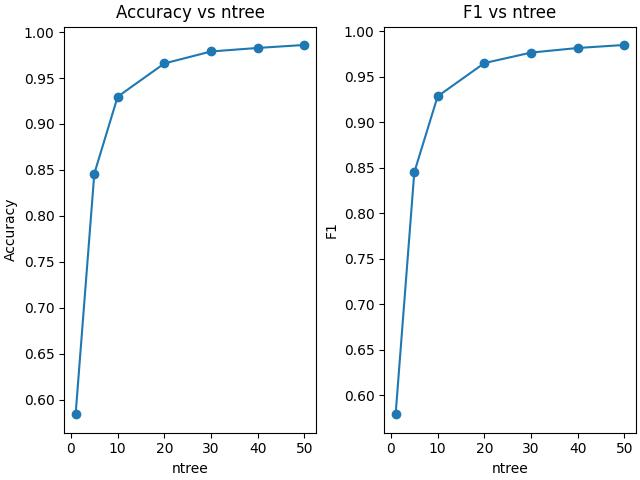
\includegraphics[width=\textwidth]{figures/forest_digits_ig.jpg}
	\caption{Random forest on Digits dataset}
	\label{fig:forest-digits}
\end{figure}

Since the datasets has many features per instance and many instances, the Decision Trees need to be more complex to be able to capture all the pattern
in the dataset. As can see from the graph, only 1 weak Decision Tree classifier performs really badly but as the number of trees increases, the accuracy
score increases and peaking at ntree = 30 while the F1 score peaks at ntree=50. The more trees are trained, the more patterns would be capture by the Random Forest since each tree
is being trained on a bootstrap subset of the original train data. So by getting the majority vote from the Random Forest, it is more likely to get
the correct prediction. Also, having only 64 numerical data is eaiser for Random Forest as at every node in the tree there would only be 2 split.

\subsection*{Neural Network}
\begin{enumerate}[label=(\alph*)]
	\item \begin{itemize}
		      \item $\lambda = 0.01$
		      \item $\alpha = 6$
	      \end{itemize}

	      \begin{table}[H]
		      \centering
		      \begin{tabular}{|l|l|l|}
			      \hline
			      Architecture      & Accuracy Score & F1 Score \\ \hline
			      {[}64 100 10{]}   & 0.946349       & 0.977977 \\ \hline
			      {[}64 40 10{]}    & 0.951350       & 0.983528 \\ \hline
			      {[}64 20 20 10{]} & 0.919259       & 0.988963 \\ \hline
		      \end{tabular}
	      \end{table}
	\item \begin{itemize}
		      \item $\lambda = 0.1$
		      \item $\alpha = 0.1$
	      \end{itemize}

	      \begin{table}[H]
		      \centering
		      \begin{tabular}{|l|l|l|}
			      \hline
			      Architecture      & Accuracy Score & F1 Score \\ \hline
			      {[}64 100 10{]}   & 0.929894       & 0.972386 \\ \hline
			      {[}64 40 10{]}    & 0.930053       & 0.972386 \\ \hline
			      {[}64 20 20 10{]} & 0.914248       & 0.966915 \\ \hline
		      \end{tabular}
	      \end{table}
\end{enumerate}

\begin{figure}[H]
	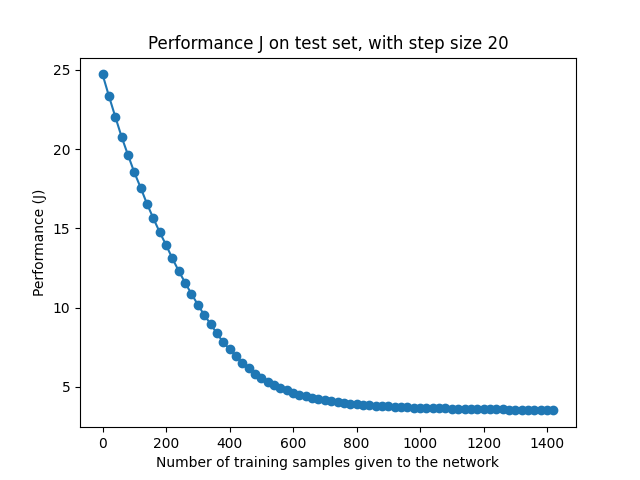
\includegraphics[width=\textwidth]{figures/nn_digits_cost.png}
	\caption{Cost J against the number of instances introduced with $\lambda=0.01, \alpha=1$ and architecture [64, 40, 10]}
	\label{fig:nn-digits}
\end{figure}

The dataset has the trend that more layers means less accuracy but it can be offset with enough neurons per layer, as with the same number of layers
the more neurons the network has, the better it performs. Having a larger $\lambda$ results in a higher performance overall while $\alpha$ values does
not have the same magnitude of impact because the $\alpha$ values is halfed as more instances is introduced to the instances. Since the dataset has
so many datasets, that means the $\alpha$ values would converge to a small number so the final weight of the network would be similar. As expected,
the more instances are introduced to the network, the cost J decreases as the weight is updated to better suited the dataset until it converges to a
small number (almost constant).

\subsection{Titanic Dataset}
We remove the name column from the dataset as we think that information does not really help to classify the result. We also one hot encode the categorical
attributes.

\subsection*{Random Forest}
\begin{itemize}
	\item \text{Split criterion: Information Gain}
	\item $min\_size\_split = 11$
	\item $min\_gain = 0.01$
	\item $max\_depth = 12$
\end{itemize}

\begin{figure}[H]
	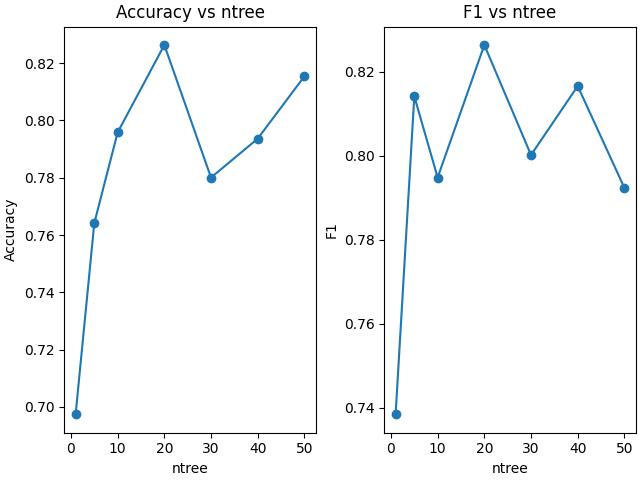
\includegraphics[width=\textwidth]{figures/forest_titanic.csv_ig.jpg}
	\caption{Random forest on Titanic dataset}
	\label{fig:forest-titanic}
\end{figure}

Since the dataset is a fairly complicate dataset with both numerical and categorical, the more complex the model is the better. As seen from the graph
ntree from 20 to 50 is the better performer compared to ntree < 20 in both accuracy and F1 score. There are less features and with less instance than
the digits datasets, so there is generally less pattern to learn from, hence a lower score overall.

\subsection*{Neural Network}
\begin{enumerate}[label=(\alph*)]
	\item \begin{itemize}
		      \item $\lambda = 0.01$
		      \item $\alpha = 6$
	      \end{itemize}

	      \begin{table}[H]
		      \centering
		      \begin{tabular}{|l|l|l|}
			      \hline
			      Architecture    & Accuracy Score & F1 Score \\ \hline
			      {[}7 40 2{]}    & 0.814128       & 0.816573 \\ \hline
			      {[}7 20 20 2{]} & 0.825092       & 0.804512 \\ \hline
		      \end{tabular}
	      \end{table}
	\item \begin{itemize}
		      \item $\lambda = 0.1$
		      \item $\alpha = 0.1$
	      \end{itemize}

	      \begin{table}[H]
		      \centering
		      \begin{tabular}{|l|l|l|}
			      \hline
			      Architecture    & Accuracy Score & F1 Score \\ \hline
			      {[}7 40 2{]}    & 0.792344       & 0.781514 \\ \hline
			      {[}7 20 20 2{]} & 0.803214       & 0.792344 \\ \hline
		      \end{tabular}
	      \end{table}
\end{enumerate}

\begin{figure}[H]
	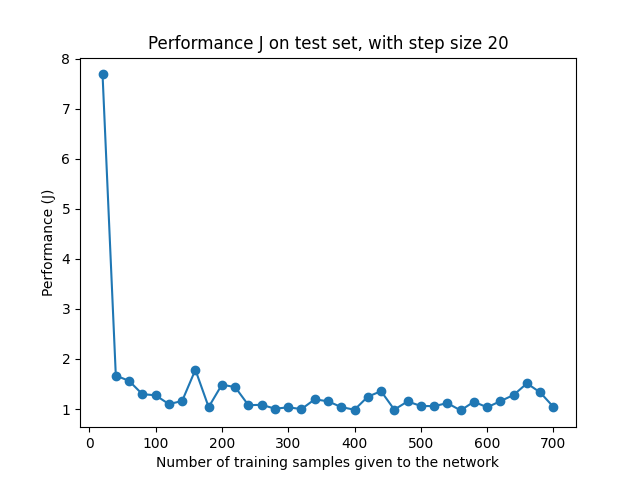
\includegraphics[width=\textwidth]{figures/nn_titanic.csv_cost.png}
	\caption{Cost J against the number of instances introduced with $\lambda=0.01, \alpha=6$ and architecture [7, 40, 2]}
	\label{fig:nn-titanic}
\end{figure}

The same trends of more layers means less performance but it can be offset with enough neurons. However in this case, too much neurons
may leads to overfitting since there are only 7 features. But with the optimal $\lambda$ it may reduce the overfitting of the network.
As a result we get an overall relatively equal score for different hyper parameters set.

\subsection{Loan Dataset}

We remove the LOAN\_ID column from the dataset as we think that information does not really help to classify the result. We also one hot encode the categorical
attributes.

\subsection*{Random Forest}
\begin{itemize}
	\item \text{Split criterion: Information Gain}
	\item $min\_size\_split = 12$
	\item $min\_gain = 0.01$
	\item $max\_depth = 12$
\end{itemize}

\begin{figure}[H]
	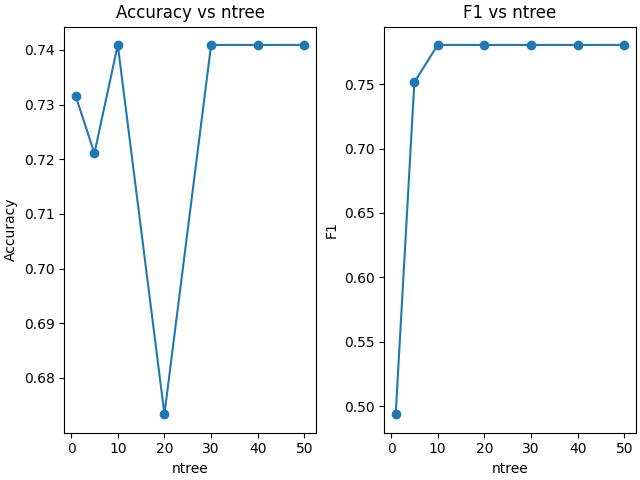
\includegraphics[width=\textwidth]{figures/forest_loan.csv_ig.jpg}
	\caption{Random forest on Loan dataset}
	\label{fig:forest-loan}
\end{figure}

While F1 score increases as ntree increases until it reaches a constant, accuracy score seems more unclear about its trends. The accuracy for
ntree = 20 really took a dip then increases back up so we are not really sure why. This dataset is a complicated one with more categorical attributes
than numerical attributes. This could be the factor contributing to the lower score when compared to the Titanic dataset as well as the inconsistancy
in accuracy score as a function of ntree.

\subsection*{Neural Network}
\begin{enumerate}[label=(\alph*)]
	\item \begin{itemize}
		      \item $\lambda = 0.01$
		      \item $\alpha = 6$
	      \end{itemize}

	      \begin{table}[H]
		      \centering
		      \begin{tabular}{|l|l|l|}
			      \hline
			      Architecture     & Accuracy Score & F1 Score \\ \hline
			      {[}18 4 2{]}     & 0.740908       & 0.780337 \\ \hline
			      {[}18 20 2{]}    & 0.740908       & 0.780337 \\ \hline
			      {[}18 20 20 2{]} & 0.731523       & 0.682143 \\ \hline
		      \end{tabular}
	      \end{table}
	\item \begin{itemize}
		      \item $\lambda = 0.1$
		      \item $\alpha = 0.1$
	      \end{itemize}

	      \begin{table}[H]
		      \centering
		      \begin{tabular}{|l|l|l|}
			      \hline
			      Architecture     & Accuracy Score & F1 Score \\ \hline
			      {[}18 20 2{]}    & 0.740908       & 0.780337 \\ \hline
			      {[}18 20 20 2{]} & 0.740908       & 0.780337 \\ \hline
		      \end{tabular}
	      \end{table}
\end{enumerate}

\begin{figure}[H]
	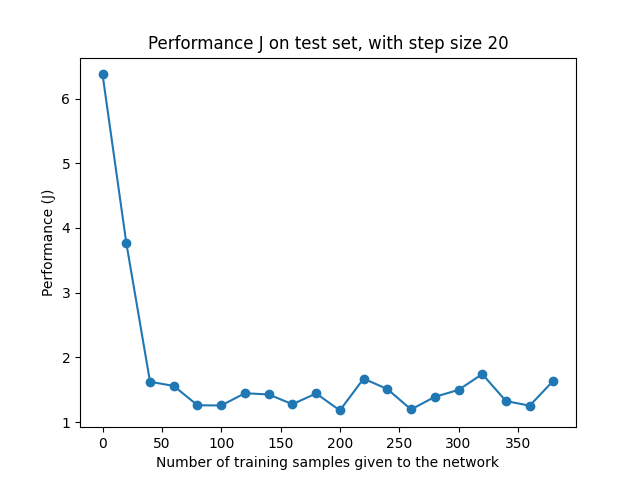
\includegraphics[width=\textwidth]{figures/nn_loan.csv_cost.png}
	\caption{Cost J against the number of instances introduced with $\lambda=0.01, \alpha=6$ and architecture [18, 20, 2]}
	\label{fig:nn-loan}
\end{figure}

For this dataset, the accuracy and F1 score for 1 and 2 hidden layers seems to converge given small enough starting $\alpha$ values. It still has the
trend that more layers means less performance, but it no longer has the property that more neurons can offset this. Rather, the scores seems to be
capped. Probably because of the many categorical attributes that is one hot encode that is causing the converging of accuracy score and F1 score
since all of its are 1 and 0 values.

\subsection{Parkinsons Dataset}

\end{document}
